% !TeX program = pdfLaTeX
\documentclass[12pt]{article}
\usepackage{amsmath}
\usepackage{graphicx,psfrag,epsf}
\usepackage{enumerate}
\usepackage{natbib}
\usepackage{textcomp}
\usepackage[hyphens]{url} % not crucial - just used below for the URL
\usepackage{hyperref}
\providecommand{\tightlist}{%
  \setlength{\itemsep}{0pt}\setlength{\parskip}{0pt}}

%\pdfminorversion=4
% NOTE: To produce blinded version, replace "0" with "1" below.
\newcommand{\blind}{0}

% DON'T change margins - should be 1 inch all around.
\addtolength{\oddsidemargin}{-.5in}%
\addtolength{\evensidemargin}{-.5in}%
\addtolength{\textwidth}{1in}%
\addtolength{\textheight}{1.3in}%
\addtolength{\topmargin}{-.8in}%

%% load any required packages here



% Pandoc citation processing

\usepackage{booktabs}
\usepackage{longtable}
\usepackage{array}
\usepackage{multirow}
\usepackage{wrapfig}
\usepackage{float}
\usepackage{colortbl}
\usepackage{pdflscape}
\usepackage{tabu}
\usepackage{threeparttable}
\usepackage{threeparttablex}
\usepackage[normalem]{ulem}
\usepackage{makecell}
\usepackage{booktabs}
\usepackage{longtable}
\usepackage{array}
\usepackage{multirow}
\usepackage{wrapfig}
\usepackage{float}
\usepackage{colortbl}
\usepackage{pdflscape}
\usepackage{tabu}
\usepackage{threeparttable}
\usepackage{threeparttablex}
\usepackage[normalem]{ulem}
\usepackage{makecell}
\usepackage{xcolor}

\begin{document}


\def\spacingset#1{\renewcommand{\baselinestretch}%
{#1}\small\normalsize} \spacingset{1}


%%%%%%%%%%%%%%%%%%%%%%%%%%%%%%%%%%%%%%%%%%%%%%%%%%%%%%%%%%%%%%%%%%%%%%%%%%%%%%

\if0\blind
{
  \title{\bf Causal Inference in Population Trends: Searching for
Demographic Anomalies in Big Data}

  \author{
        Mathew E. Hauer \\
    Department of Sociology, Florida State University\\
     and \\     Stephanie A. Bohon \\
    Department of Sociology, University of Tennessee - Knoxville\\
      }
  \maketitle
} \fi

\if1\blind
{
  \bigskip
  \bigskip
  \bigskip
  \begin{center}
    {\LARGE\bf Causal Inference in Population Trends: Searching for
Demographic Anomalies in Big Data}
  \end{center}
  \medskip
} \fi

\bigskip
\begin{abstract}
The proliferation of big data, wider access to advanced computing
platforms, and the development of powerful statistical algorithms can
uncover hidden anomalies in social data, previously dismissed as noise.
Here, we combine causal inference techniques and abductive reasoning to
identify fertility and mortality anomalies on twenty years of complete
demographic data in the United States. We uncover real, ``hidden'' baby
booms/busts and mortality spikes/dips, distinguishable from regular
trend variations. We identify more than 22 and 156 fertility and
mortality anomalies, totaling more than 200k and 600k anomalous births
and deaths, respectively. Notable detectable mortality anomalies include
the September 11 2001 terrorist attack in New York and the emergence and
acceleration of the opioid epidemic in New Hampshire. Notable fertility
anomalies include the ``missing births'' in Louisiana after Hurricane
Katrina and the reduction in fertility behavior after the September 2008
stock market crash in Connecticut, amongst others. The combined causal
inference and abductive reasoning approach can be readily adapted to
find other, undiscovered social phenomena or to evaluate the efficacy of
important public policies.
\end{abstract}

\noindent%
{\it Keywords:} mortality, fertility, causal inference, abductive
reasoning, big data
\vfill

\newpage
\spacingset{1.45} % DON'T change the spacing!

\newpage

\hypertarget{introduction}{%
\section{Introduction}\label{introduction}}

The search for causality is one of the primary motivations of social
scientists \citep{smith2011commentary, pearl2009causal}. Causal
inference, the identification of causal effects, attempts to uncover the
underlying mechanisms that result in changes in a phenomenon and has a
long history as an approach to inquiry in the social sciences
\citep{grimmer2015ppsp}. Often, the identification of a casual mechanism
is accomplished via a randomized control trial (RCT) or expert knowledge
applied to a natural experiment \citep{salganik2019bit}.

Unfortunately, both RCTs and natural experiments have drawbacks. RCTs
are often prohibitively expensive for many scientists, precluding their
widespread adoption in the social sciences \citep{west2008ajph}. RCTs
are also sometimes impossible to deploy in the ``real world.'' For
instance, an RCT to study country-level austerity measures would be
difficult, if not impossible, to implement. RCTs to study fertility
would be immoral. Natural experiments are a cheaper alternative but
provide less certainty about causation, fewer opportunities to replicate
work, and require expert knowledge of the natural experiment to be
properly employed \citep{pearl2018book}.

Additionally, both RCTs and natural experiments are based on traditional
hypothesis-based testing, the deductive scientific paradigm where a
question is first posed and scientists generate or find data to answer
the question. Such approaches, while extensively utilized and
time-tested, increase the likelihood that a researcher will miss
important phenomena that might go unnoticed because it falls outside the
hypothesis, or the study could suffer from extensive p-hacking
\citep{head2015extent, nuzzo2014scientific, ruggles2014big}. At the same
time, purely inductive data mining can result in false assertions or
spurious findings, especially in the hands of those who are not field
experts \citep{yanai_hypothesis_2020}. Abductive reasoning, sometimes
described as ``inferring cause from effect'' \citep{Crowder2017}, moves
the scientific process from the inductive to the deductive, and
sometimes back and forth, to reach conclusions \citep{bryant2014realm}.
Physical scientists use abductive reasoning more commonly than social
scientists. The discovery of Neptune in 1846 based on unexplained
perturbations of the orbit of Uranus \citep{popper2005logic}, the
discovery of galactic migration of planets \citep{gomes2005n}, and the
current generation of gravitational wave detectors such as the Laser
Interferometer Gravitational-Wave Observatory (LIGO)
\citep{harry2010advanced} demonstrate the power of the abductive
approach in the physical sciences.

In a data-rich environment, abductive reasoning can be more easily
applied to first find effects and then infer their cause ex-post. The
modern proliferation of data, advances in high performance (``super'')
computing, and the development of powerful statistical algorithms
provide an environment ripe for wedding causal inference with abductive
reasoning \citep{van2016data, zikopoulos2011}, with the potential for
researchers to find hidden or understudied social phenomena
\citep{bohon2018demography}. While the availability of big data and high
performance computing allows novel exploration of data through causal
inference
\citep{bohon2018demography, rcausalimpact, shiffrin2016drawing},
relatively few studies utilize causal inference techniques in the study
of demographic phenomena. However, understanding social phenomena using
these advances reveals important insights into society
\citep{angrist1989lifetime, mas2009peers} and allows us to better
monitor population trends \citep{nobles2019, torche2015hidden}. The rich
demographic data available in the United States make the potential
revelation of interesting and important demographic phenomena not only
possible, but extremely plausible -- even if identification of the
phenomena occurs without identifying the underlying cause.

In this paper, we combine a modern statistical outlier detection
algorithm \citep{chen1993joint}, abductive reasoning, and large
demographic data sets on more than 20 years of mortality and fertility
trends to identify anomalous demographic behavior. In essence, we
identify \emph{effects without knowledge of the cause}. We ask one
fundamental question regarding demographic anomalies: What are the
hidden baby booms/busts and mortality spikes/dips in the United States
over the last twenty years? We do not necessarily know the causes of
these anomalies and suggest causes for select anomalies. Even without
knowledge of the causes, simply identification of anomalies allows
scientists with more detailed knowledge of local population dynamics,
state-level policy making, or macro-economics to explain these phenomena
post-hoc. From explanations of phenomena that may have previously gone
unnoticed, social scientists may be able to better forecast populations
and provide policy solutions for impending problems such as climate
change.

\hypertarget{abductive-reasoning-and-causal-inference}{%
\section{Abductive Reasoning and Causal
Inference}\label{abductive-reasoning-and-causal-inference}}

Scientific inquiry falls under one of three modes of logical reasoning:
deduction, induction, and abduction. Deductive reasoning starts with a
theory and makes a prediction of what the observations should be if that
theory is correct. The classic example of deductive reasoning
essentially goes (a) ``all men are mortal,'' (b) ``Socrates is a man,''
(c) ``therefore, Socrates is mortal.'' Deductive reasoning has a long
history in the sciences and most hypothesis testing in the social
sciences follows this logical reasoning. For example, John Snow used
deductive reasoning to stop the 1854 London cholera outbreak. He
hypothesized that cholera was waterborne and deduced that a bad water
pump was responsible for the outbreak.

Inductive reasoning is directionally opposite of deductive reasoning.
Rather than starting with a theory and making a prediction, induction
starts with an observation and makes a theory based on the likeliest
reason. For example, the Hispanic Mortality Paradox first appeared in
the scientific literature in the mid-1980s \citep{markides1986health} as
an observation that Hispanics in the United States had better health
outcomes than expected given their socioeconomic status. Based on this
observation, numerous theories arose to explain this paradox.

Both deductive and inductive reasoning are well established in science
but are not without their shortcomings. In both approaches, it is
impossible, or at least improbable, for the premise to be true and the
conclusion false. Furthermore, if a hypothesis is rejected under a
deductive or inductive approach, there is no alternative explanation --
there is either the presence or absence of support.

Abductive reasoning is a third, less well-known way that reasons the
best explanation given the observations \citep{walton2014abductive}. It
is most concerned with generating and evaluating explanatory hypotheses
\citep{Crowder2017} by looking for a pattern and suggesting a hypothesis
\citep{fann2012peirce, pierce1878deduction}. Unlike the more rigid
deductive and inductive reasoning, abductive reasoning allows the
scientist to move between deduction and induction and fits well during
exploratory data analysis
\citep{yu1994abduction, haig2015commentary, tukey1977exploratory}.
During exploratory data analysis, abductive reasoning helps find a
pattern and suggest a hypothesis, deduction helps refine and build a
testable hypothesis, and induction is the empirical support
\citep{yu1994abduction}.

Abductive reasoning and exploratory data analysis are best employed in a
data rich environment -- the very data environment social scientists and
demographers find themselves in the present moment. In a data rich
environment, a hypothesis is a hidden liability
\citep{yanai_hypothesis_2020} because it focuses our attention on only
that which we seek. To demonstrate this, \footnote{Yanai and Lercher
  \citeyearpar{yanai_hypothesis_2020} ask if focusing on a specific
  hypothesis prevents new discovery. By way of illustration, they
  created a simple dataset that if plotted would reveal an image of a
  gorilla waving. Students instructed to find support for specific
  hypotheses were less likely to discover the gorilla compared to those
  who were simply asked ``What do you conclude from the dataset?''}.
Focusing on specific hypotheses often prevents us from finding other
interesting phenomena. After all, it was the publication of the Hispanic
paradox itself that has generated more than thirty years of devoted
scholarship. At the same time, when paired with causal inference
techniques, abductive reasoning provides an empirical platform for the
discovery of potentially interesting social phenomena; it provides an
important tool for sifting large amounts of data to find interesting
results without the blinders of hypothesis testing.

\hypertarget{materials-and-methods}{%
\section{Materials and Methods}\label{materials-and-methods}}

\hypertarget{method}{%
\subsection{Method}\label{method}}

We use a statistical time series outlier detection algorithm
\citep{chen1993joint}, implemented in the R programming language
\citep{rcore} via the tsoutliers package \citep{tsoutliers2019}. This
algorithm iteratively uses ARIMA models to 1) identify potential
outliers or anomalies and 2) refit the ARIMA with the outliers removed
to produce a counter-factual time series. Here we briefly summarize and
describe the method.

Often, the behavior of a time series can be described and summarized in
ARIMA models. If a series of values, \(y_t^*\), is subject to \(m\)
interventions or outliers at time points \(t_1,t_2,…,t_m\) with weights
\(\omega\) then \(y_t^*\) can be defined as

\begin{equation}
\label{eq:arima}
y_t^* = \sum_{j=1}^{m} \omega_jL_j(B)I_t(t_j) + \frac{\theta(B)}{\phi(B)\alpha(B)}\alpha_t 
\end{equation}

Where \(I_t(t_j)\) is an indicator variable with a value of 1 at
observation \(t_j\) and where the \(j\)th outlier arises,\\
\(\phi(B)\) is an autoregressive polynomial with all roots outside the
unit circle,\\
\(\theta(B)\) is a moving average polynomial with all roots outside the
unit circle,\\
and \(\alpha(B)\) is an autoregressive polynomial with all roots on the
unit circle.

We examine three types of outliers at time point \(t_m\):\\
1. additive outliers (AO), defined as \(L_j(B)=1\);\\
2. level shift outliers (LS), defined as \(L_j(B) = 1/(1-B)\); and\\
3. temporary change outliers (TC), defined as
\(L_j(B) = 1/(1-\delta B)\) where \(\delta\) is equal to 0.7.

Colloquially, additive outliers arise when a single event causes the
time series to unexpectedly increase/decrease for a single time period;
level shift outliers arise when an event causes the time series to
unexpectedly increase/decrease for multiple time periods; and temporary
change outliers arise when an event causes the time series to
unexpectedly increase/decrease with lingering effects that decay over
multiple time periods.

An outlier is detected with the estimated residuals using a regression
equation

\begin{equation}
\label{eq:residuals}
\pi(B)y_t^* \equiv \hat{e} = \sum_{j=1}^m \omega_j \pi(B)L_j(B)I_t(t_j) + \alpha_t
\end{equation} where \(\pi(B)=\sum_{i=o}^{inf} \pi_iB^i\).

Equations \ref{eq:arima} and \ref{eq:residuals} allow for an automatic
detection of anomalies iterated over a two-stage process.

In stage 1, anomalies are located. First, an ARIMA model is fit to the
time series using the \texttt{forecast} package in R
\citep{Rforecast, hymdman2008} where the best performing ARIMA model is
selected based on the Bayesian information criterion (BIC). Next, the
residuals from the forecast are checked for their significance using
equation \ref{eq:residuals} where only anomalies above a critical
\emph{t}-static are considered ``true'' anomalies (\(|\tau| \geq 3.5\)).
We choose this critical value based on Chen and Liu's
\citeyearpar{chen1993joint} recommendation to minimize Type I or
false-positive anomalies. Finally, two additional rules are implemented:
If multiple anomalies are detected at the same time point, only the most
significant anomaly is selected and if anomalies of the same type at
consecutive time periods are detected, only the anomaly with highest
\emph{t}-statistic is selected.

In stage 2, anomalies are removed from the time series and a new ARIMA
model is chosen and fit. The selection of the initial ARIMA model could
have been affected by the presence of the anomalies, making some
anomalies spuriously identified. To correct for this, a new ARIMA model
is fit accounting for additional regression effects in equation
\ref{eq:arima} from the list of candidate anomalies identified in stage
1, effectively removing the anomalies from the time series. Each anomaly
is then reassessed under the new model and those anomalies that are no
longer significant are removed.

These two stages are then iterated until no additional anomalies are
detected.

\begin{figure}
\centering
\includegraphics{MainDocument_files/figure-latex/ToyExample-1.pdf}
\caption{\textbf{An example of anomaly detection using Hurricanes Katrina and Rita in Orleans Parish Louisiana in 2005.}
Hurricane Katrina struck Louisiana in 2005 and we use it as a toy
example to illustrate our approach. This figure shows the annual time
series of total population in Orleans Parish between 1980 and 2019.
Between 1990 and 2005, Orleans Parish total population changed from 495k
to 494k, suggesting a possible `plateau' in the population (illustrated
with the dotted `counterfactual'). Hurricane Katrina and the widespread
population loss of more than 200k people represent a very strong anomaly
(t=-96.39) \label{explanationfigure}}
\end{figure}

\hypertarget{toy-example}{%
\subsection{Toy example}\label{toy-example}}

\textbf{\autoref{explanationfigure}} shows a toy example for anomaly
detection in a time series using the example of Hurricane Katrina in
Orleans Parish. On August 23 2005, Hurricane Katrina, a category 5
hurricane, struck southern Louisiana causing widespread damage and
destruction in Orleans Parish in particular. The displacement from the
Hurricane and the federal response were well documented
\citep{horiDisplacementDynamicsSouthern2009, fussellRecoveryMigrationCity2014}
and Census estimates suggest Orleans Parish lost more than 200,000
residents between 2005 and 2006. What would have been Orleans'
population estimate had Hurricane Katrina \emph{not} occurred? A simple
counter-factual estimate might keep population size just under 500,000
people (\(\hat{y}\)).

In the Hurricane Katrina example, we have knowledge of the impact of
Hurricane Katrina after the fact or ex-post-facto in order to create the
counter-factual time series \(\hat{y}\). But is this anomaly detectable
without knowledge of the Hurricane Katrina? In other words, can we
detect the reduction of Orleans Parish's population between 2005 and
2006 using only the time series? Absolutely. the tsoutliers package
identifies 2006 as an extremely strong level-shift outlier
(\emph{t}-stat = -96.39). The real world is hardly this simplified where
a direct intervention is known, is large, and is testable.

\hypertarget{data}{%
\subsection{Data}\label{data}}

We search for demographic anomalies using the Center for Disease Control
and Prevention's online WONDER monthly fertility (2003-2017) and
mortality databases (1999-2016) for all fifty states and the District of
Columbia \citep{CDC_fert07, CDC_mort}. These data sets contain every
birth and death record in the United States over the time periods of
interest, representing the universe of both mortality and fertility data
in the US. These data are considered the ``gold standard'' of data
collections \citep{mahapatra2007civil} and have been considered
``complete'' since 1968 \citep{hetzel2016us}. We search over each state
equivalent's (n=51) mortality (n=228) and fertility (n=180) monthly time
series for a total of 20,808 state-months of data.

\hypertarget{robustness-check}{%
\subsection{Robustness Check}\label{robustness-check}}

Chen and Liu \citeyearpar{chen1993joint} report results of a simulation
exercise of varying critical value levels. They simulated various
anomaly-free time series and injected specific anomalies of varying
\(\sigma\) levels. For a critical value of 3.5 -- the level Chen and Liu
recommend to minimize both false-positive (Type I) and false-negative
(Type II) error rates -- they report Type I error rates between 0.0\%
and 0.1\% and Type II error rates or the statistical power between 40\%
and 60\% with injected anomalies equal to 4\(\sigma\). We follow their
lead by simulating time series to test for Type I and Type II errors. We
base our simulation on the 41 time series that do not contain any
anomalies (see \textbf{Results} below; 33 without a single fertility
anomaly and 8 without a single mortality anomaly).

To test for false-positive rates, we simulate 1000 time series for each
of the 41 state-components (fertility or mortality) using the fitted
ARIMA model for each state-component. This allows the simulated time
series to mimic the underlying true time series (see
\textbf{Supplementary Material} for the underlying code). Any anomalies
we detect in the 7,764,000 candidate time steps are spurious anomalies.
We detect 6,588 anomalies for a false-positive error rate of 0.085\%.

To test for false-negative rates, we use the underlying true,
sans-anomaly time series but introduce a single anomaly (magnitude equal
to 3.5\(\sigma\)) at the same time point in each series. If the
\texttt{tsoutliers} algorithm fails to detect the anomaly, it would be
considered a false-negative error. We detect 27,904 out of 41,000
candidate time series giving us a false-negative error rate of 31.9\%.
This provides a statistical power of 68.1\%.

Based on these tests we think it is clear that our probability of
committing a Type I error (or claiming an anomaly is true when in fact
is not) is very low. But, based on our false-negative error rate, it is
possible that the anomalies we do detect are \emph{conservative}. Our
statistical power is of just 68.1\% suggests a higher than normal
likelihood that true effects are going undetected. We are unlikely to
commit an error of commission (ie, including a false anomaly) but are
more likely to commit an error of omission (ie omitting true anomalies).
Thus our results should be considered conservative.

\hypertarget{replication-files}{%
\subsection{Replication Files}\label{replication-files}}

All data and code necessary to reproduce the reported results are
licensed under the CC-BY-4.0 license and are publicly available as
\url{https://osf.io/yc3r4/?view_only=3ce3ca267c7047e0942940ebd08846d0}.
The analyses were performed in \emph{R} \citep{rcore}.

\hypertarget{results}{%
\section{Results}\label{results}}

We detect numerous anomalous mortality and fertility events at the US
state-level since 1999. A full listing of these anomalies can be found
in the \textbf{Supplementary Materials}. We begin by highlighting
significant fertility and mortality anomalies across all three types of
outliers (Additive Outliers, Level Shift Outliers, and Temporary Change
outliers) with plausible explanations. We then highlight two strong
anomalies that belie explanation. Finally, we conclude with a summary of
the anomalies we detect.

\hypertarget{fertility}{%
\subsection{Fertility}\label{fertility}}

We begin with a clear temporary change (TC) outlier for fertility in
Louisiana (\textbf{\autoref{fig:fertla}a}). Here we detect two TC
outliers, nearly back-to-back in 2005 (2005:08 \emph{t} = -6.002; and
2005:10 \emph{t} = -4.997), coinciding with the destruction of Hurricane
Katrina from the same year. The migration associated with Hurricane
Katrina has garnered most of the attention of social scientists
\citep{fussellRecoveryMigrationCity2014, horiDisplacementDynamicsSouthern2009},
but the hurricane had a very clear impact on fertility behaviors too,
creating a mini ``baby bust'' in Louisiana with the departure of many
people in their childbearing years. We estimate 4,411 fewer births in
Louisiana compared to the counter-factual, likely attributable to the
Hurricane.

We also highlight a level shift (LS) outlier for fertility in
Connecticut. Here we detect a strong (\emph{t}= -3.71 for -285
births/month) level shift toward lower fertility beginning in August
2009 (2009:08) that continues through the end of the period
(\textbf{\autoref{fig:fertla}b}). This LS toward lower fertility reduced
the number of births by 28,752 or 9\%) lower than the counter-factual
time series. The stock market crash of 2008, where the Dow Jones
Industrial Average had the largest single-day loss up to that point,
occurred just 11 months before we detect a shift toward lower fertility.
It is possible that the trend toward lower fertility in August 2009 and
the stock market crash in September 2008 are linked, although, as stated
previously, we are speculating only to illustrate how causal inference
could work in an abductive research agenda. A potentially interesting
future line of research would be to link fertility anomalies to the
kinds of economic shocks that may lead to out-migration of those in
their childbearing years.

\begin{figure}
\centering
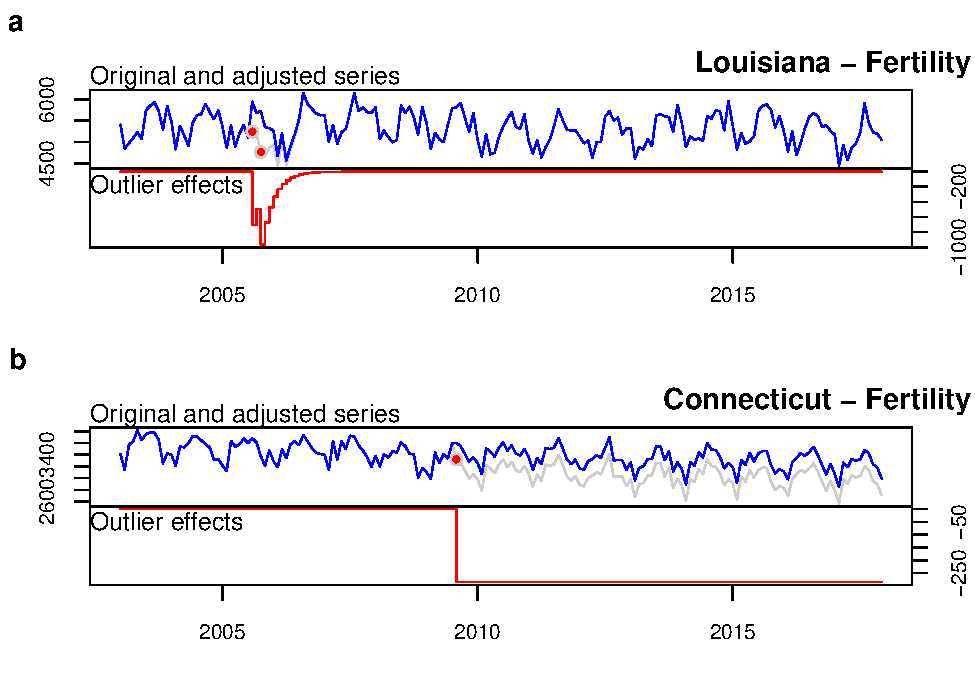
\includegraphics{MainDocument_files/figure-latex/FertilityAnomalies-1.pdf}
\caption{\textbf{Anomaly detection in Louisiana (a) and Connecticut (b) state fertility, 2003-2018.}
The top part of each panel contains the original time series (light
gray), the adjusted, counter-factual time series in the absence of
anomalies (blue), and the red dots correspond to the onset of detected
anomalies. The bottom part of each panel contains the magnitude and type
of the outlier in red. In (a), we detect two outliers, back-to-back,
likely resulting from Hurricane Katrina in August and October 2005,
representing a decrease of more than 4,400 births due to the hurricane
(t-statistics= -6.002 and -4.997). In (b), we detect one outlier, a
level shift outlier (LS) in August 2009. We believe this reduction is
attributable to the stock market crash 11 months earlier (t-statistic =
-3.71). \label{fig:fertla}}
\end{figure}

\hypertarget{mortality}{%
\subsection{Mortality}\label{mortality}}

For mortality, we will use New York State as an example
(\textbf{\autoref{fig:mortnewhamp}a}). We identify seven anomalies in
the mortality time series for New York, all with \emph{t}-statistics in
excess of 3.91, making these anomalies unlikely to be due to chance. The
algorithm correctly identifies September 2001 as an additive outlier
(2001:09 \emph{t}= 6.396) where there were 1,628 more deaths in that
month than anticipated. This mortality event is likely caused by the
September 11 terrorist attack on the World Trade Center that immediately
killed 2,606 people and the detection of this mortality event provides
confidence in our detection of other anomalies.

In \textbf{\autoref{fig:mortnewhamp}a}, notice the strong level shift
(LS) that occurs in February 2004 (2004:02 \emph{t}= -5.594) which
prevented 869 deaths per month. This shift totals more than 144,000
averted deaths compared to the counter-factual time series and is the
single largest mortality protective anomaly among all states. This
translates to 7\% fewer deaths than expected over the time period. What
is driving this mortality protection? What policies did NY put into
place that might have contributed to this considerable mortality
reduction? What environmental or economic conditions may have changed?
These are the kinds of questions that arise from our analyses. The
purpose of our paper is not to answer these questions, but our findings
underscore the need for more research that takes an abductive approach.
By identifying anomalies through an inductive process, researchers can
then look for underlying causes. Once those causes are identified,
researchers can then use a deductive process to see if such events
predict other (or future) anomalies.

To see the potential for combining abductive reasoning with causal
inference, contrast the mortality protection in New York with the
enhanced mortality in New Hampshire
(\textbf{\autoref{fig:mortnewhamp}b}). In New Hampshire we detect two
significant level shifts (LS) in the monthly mortality data, first in
April 2010 and again in November 2014 (2010:04 \emph{t}= 3.51; 2014:11
\emph{t}= 6.68). These anomalies suggest New Hampshire experienced 8,159
more deaths (+9\% more than expected) in a seven-year period beginning
in early 2010. These are events not experienced by neighboring states
during the same time period, and this is the single largest percentage
mortality increase/decrease we detected among all states. Not
coincidentally, NH has the second highest opioid-related mortality in
the US \citep{beetham2019access} and it is likely that we detect this
epidemic in our results. Isolating these anomalies and testing them
against opioid sales data might yield intriguing results.

\begin{figure}
\centering
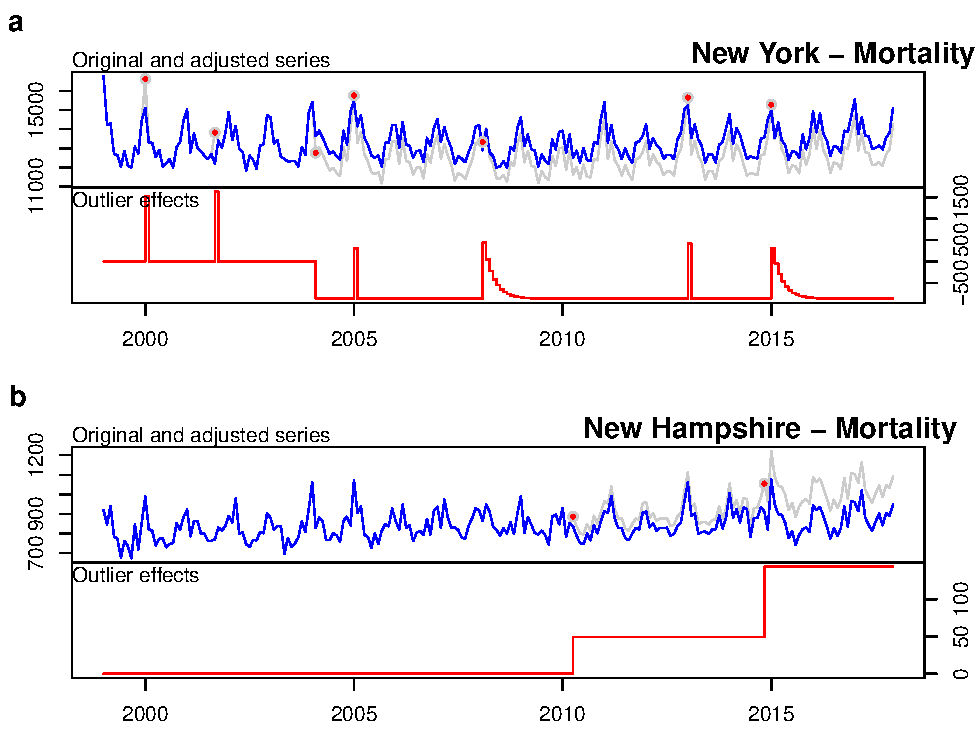
\includegraphics{MainDocument_files/figure-latex/MortalityAnomalies-1.pdf}
\caption{\textbf{Anomaly Detection for New York (a) and New Hampshire (b) state mortality, 1999-2016.}
In New York (a), we detect additive outliers (AO) in January 2000,
September 2001, January 2005, and January 2013; temporary change (TC)
outliers in February 2007 and January 2015; and a level shift (LS)
starting in February 2004. In New Hampshire (b), we detect two outliers,
both level shift outliers (LS) in April 2010 and again in November 2014.
These anomalies suggest New York experienced a significant mortality
event in September 2001 and New Hampshire experienced approximately
9,700 more deaths than expected since 2010 or 14\% more deaths in the
state over just seven years. \label{fig:mortnewhamp}}
\end{figure}

\hypertarget{interesting-anomalous-fertilitymortality-events}{%
\subsection{Interesting Anomalous Fertility/Mortality
events}\label{interesting-anomalous-fertilitymortality-events}}

In the examples above, we highlighted four fertility/mortality anomalies
with plausible explanations. In the case of New York and New Hampshire,
the mortality anomalies have plausible explanations. It seems likely
that New York's AO anomaly in September 2001 is caused by the 9/11
tragedy and the rise in New Hampshire's mortality starting in 2010 could
be linked to the opioid epidemic. Similarly, Louisiana's TC anomalies
seem linked to Hurricanes Katrina and Rita while the LS anomaly in
Connecticut's fertility appears linked to the Great Recession. However,
we detect numerous other demographic anomalies in other states, on the
causes of which we will not speculate. \textbf{\autoref{fig:ferthawaii}}
shows two such unexplained anomalies.

In \textbf{\autoref{fig:ferthawaii}a} we identify a single additive
anomaly in Hawaiian fertility in May 2014. This is a strong anomaly with
a \emph{t}-statistic of 4.96, 15\% above the counter-factual time
series. This single, anomalous month is also the second highest monthly
births in the time series. We have no plausible explanation for this
anomaly. We do not believe this is simply a data error as the other
extreme values, September 2008 and February 2005 with the highest and
lowest recorded fertility respectively, were not identified as anomalous
events. Even if we were to assume this anomaly resulted from data entry
error, it remains an \emph{unaltered} data error in the Hawaiian monthly
fertility data.

This is contrast to \textbf{\autoref{fig:ferthawaii}b}, where we
identify a strange mortality reduction in Ohio (\emph{t}-stat: -4.27).
This LS is more than 1,157 deaths per month less than the
counter-factual time series, suggesting Ohio had nearly 40,000 fewer
deaths since February 2015 than expected. This is the single-largest LS
among all states. We could not identify the potential policies Ohio
might have put into place or the events that occurred to provide such a
strong mortality protection.

\begin{figure}
\centering
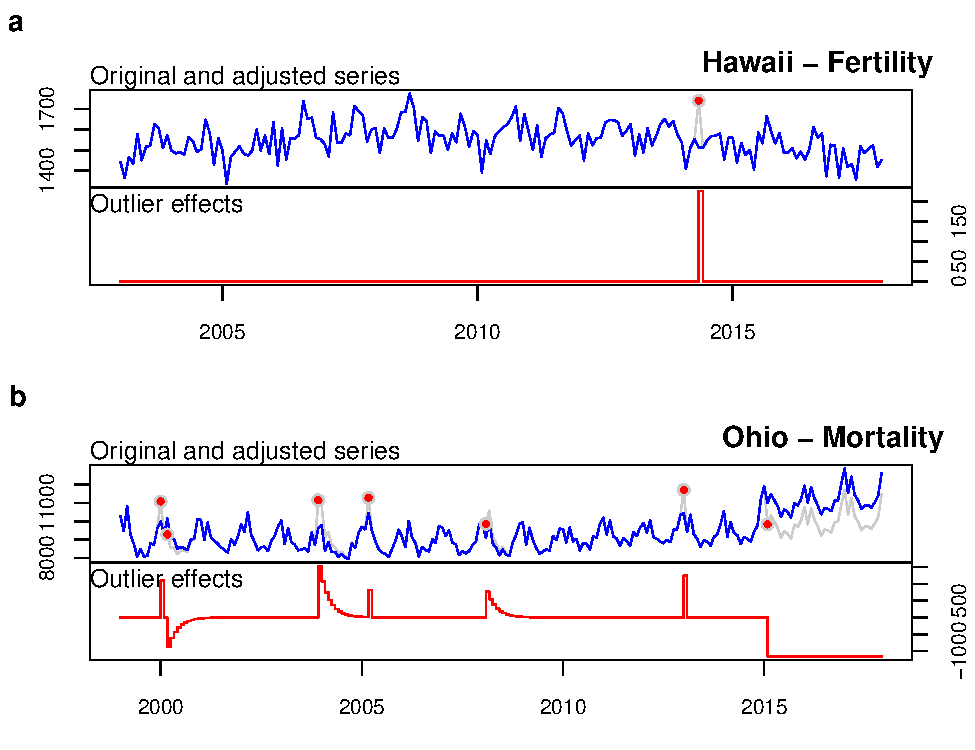
\includegraphics{MainDocument_files/figure-latex/TrueAnomalies-1.pdf}
\caption{\textbf{Anomaly detection in Hawaii state fertility (a) and Ohio state mortality (b).}
Here we detect one outlier, an additive outlier (AO) in May 2014 in
Hawaii (a), representing a large, unexplainable 14\% increase in
expected births in that month. We also detect a strong level shift (LS)
reduction (b), representing a large, unexplainable reduction of nearly
40,000 deaths in Ohio. \label{fig:ferthawaii}}
\end{figure}

\hypertarget{overall-anomalies}{%
\subsection{Overall Anomalies}\label{overall-anomalies}}

\begin{table}

\caption{\label{tab:unnamed-chunk-7}\textbf{Summary by Demographic Component.}  Here we can see there 22 Fertility and 156 Mortality anomalies among the state-level time series, totalling more than 200k anomalous births and 600k anomalous deaths. \label{sumtable}}
\centering
\begin{tabular}[t]{lrllrrr}
\toprule
Component & Anomalies & $y$ & $\hat{y}$ & $y-\hat{y}$ & $|y-\hat{y}|$ & \% of Total\\
\midrule
Fertility & 22 & 25.48M & 25.68M & -202,217 & 226,476 & 0.889\\
Mortality & 156 & 43.57M & 43.52M & 48,535 & 627,364 & 1.440\\
\bottomrule
\end{tabular}
\end{table}

\textbf{\autoref{sumtable}} reports the overall number of anomalies we
detect of each type for births and deaths and some summary statistics
across all anomaly types and \textbf{\autoref{fig:summap}} maps these
results.

We find considerably more mortality anomalies (n = 156) than fertility
anomalies (n = 22). Given that anomalies are always the product of
events \citep{song2018anomaly}, finding more mortality than fertility
anomalies is not surprising. Mortality is likely to spike in response to
a catastrophic event (like an earthquake or terrorist attack) or due to
a disease outbreak while the effects of a catastrophic event on
fertility is less predictable. One reason for this is that fertility is
linked to human decision-making more directly than mortality
\citep{stein2014couples} which results in more varied outcomes, so, for
example, researchers find that catastrophic weather events can increase
childbearing among those who already have a child, but not among the
childless \citep{Evans2008Hurricanebirth}. Some events, like the 1995
Oklahoma City bombings, resulted in both fertility and mortality
changes. However, changes in fertility manifest over a longer time
horizon after an event, and the relationship between a
fertility-inducing event and behavior change is less strong than the
relationship between a mortality-inducing event (such as a terrorist
incident) and death \citep{Rodgers2005OKBombing}. Of course, not all
events that impact fertility and mortality are catastrophic. Researchers
have documented that more commonplace events such as massive layoffs
\citep{Venkataramani2019} or policy changes
\citep{Livingston2017Cannabis} can also create anomalies in mortality
patterns, but we have not found such evidence for fertility.

Consistent with more anomalies across the time series, we find more
anomalous deaths (627,364) than anomalous births (226,476). Fertility
anomalies overwhelmingly tend toward lower fertility, with only a few
fertility anomalies yielding more births. This is consistent with
research findings that link severe weather events to significantly lower
fertility \citep{Evans2008Hurricanebirth}. Conversely, mortality
anomalies tend to be more evenly split between positive and negative
anomalies, but tend toward more deaths rather than fewer deaths. Again,
this is not surprising, as the kinds of events that increase death
(e.g., plant closings are associated with increased opioid death
\citep{Venkataramani2019}) are more common than the events that decrease
death (e.g., cannabis legalization is associated with decreased opioid
deaths \citep{Livingston2017Cannabis}). These anomalous deaths and
births account for 1.44\% and 0.889\% over the entire time series,
respectively.

As \textbf{\autoref{fig:summap}} shows, three states exhibited neither
mortality nor fertility anomalies: Alaska, North Dakota, and South
Dakota. Another nine states exhibited just a single anomaly (Delaware,
District of Colombia, Idaho, Illinois, Kansas, Nevada, New Mexico, Utah,
and Wyoming). Both New York and Massachusetts exhibited the most
anomalies with nine.

\begin{figure}
\centering
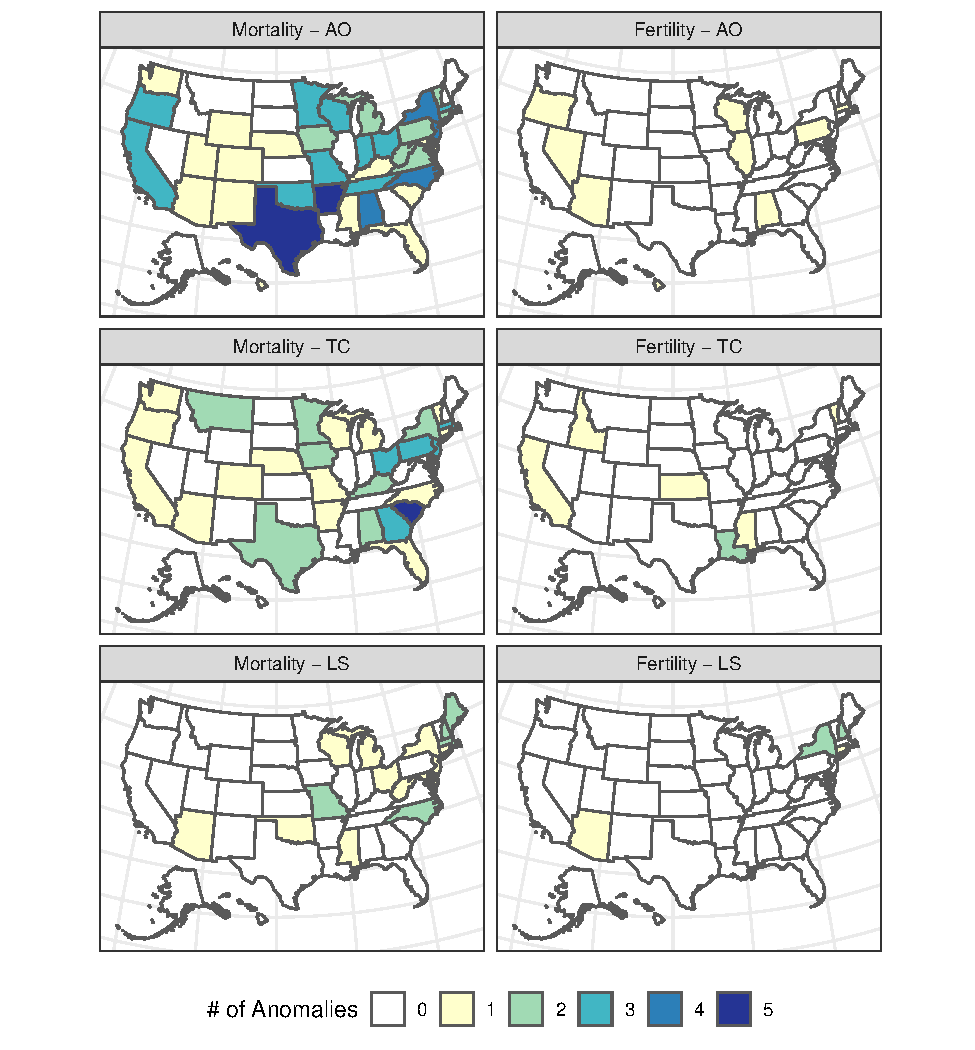
\includegraphics{MainDocument_files/figure-latex/AnomalyMap-1.pdf}
\caption{\textbf{Summary of Anomalies by type, demographic component, and State.}
We observe much fewer fertility anomalies than mortality anomalies.
\label{fig:summap}}
\end{figure}

\hypertarget{conclusion}{%
\section{Conclusion}\label{conclusion}}

Data scientists frequently claim that the big data revolution is a
turning point in scientific discovery that will allow us to solve some
of the world's most pressing problems \citep{grimmer2015ppsp}. Social
scientists are skeptical of such claims, because they better understand
the complexities of the social world and know from experience that data
alone are not enough to solve social problems
\citep{bohon2018demography, grimmer2015ppsp}. Nonetheless, the increased
availability of data and (more importantly, we argue) the development of
advanced techniques for analyzing these data will enable important
discovery \citep{monroe2015no}.

One technique that population scientists underutilize is causal
inference. Causal inference, in the simplest terms, is the discovery of
effects in search of a cause using big data and advanced computing
algorithms \citep{imai2008misunderstandings}. This inductive approach is
uncommon in quantitative social science where hypothesis testing is
expected, and approaches are largely deductive. However, common
statistical hypothesis testing is impractical with big data, as
significant p values are guaranteed, and such approaches do not allow us
to uncover all the information that big data has to offer
\citep{monroe2015no}. Here, we call for an abductive approach, where
causal inference algorithms are applied to high quality data to uncover
irregularities that are unlikely to be attributable to expected
variations in trends (or noise) as a first step to then developing
testable hypotheses about causes. Abductive approaches allow researchers
to move from the inductive to the deductive and sometimes work back and
forth in aid of scientific discovery.

In this paper, we show how the tsoutlier package in R can be implemented
to conduct statistical time series outlier detection, an inductive
approach that aids in the creation of deductive reasoning. This
algorithm is one of many causal inference approaches that are freely and
commercially available (see \citet{rcausalimpact}). In our initial work,
we experimented with other approaches, such as Google's CausalImpact
algorithm, which uncovered the same patterns we briefly discuss in this
paper. By making more use of causal inference techniques and abductive
modeling approaches, we argue that social scientists will be able to
better understand how events or policy implementation can impact
important outcomes. For example, we could uncover---on a wide
scale---how gun control policies may reduce or increase injuries from
shootings or how marijuana legalization might impact opioid deaths. We
could also uncover how increases in extreme weather events impact a
range of behaviors such as home sales, bottled water purchases, and even
fertility.

In our demonstration, we show how the application of causal inference to
state-level time series fertility and mortality data uncovers three
types of demographic anomalies: those that occur and disappear quickly,
those that occur and decay over time, and those that occur and remain.
Uncovering these anomalies in and of themselves is important. For
example, the algorithm we deploy clearly shows the fertility effects of
Hurricanes Katrina and Rita as well as the mortality effects of the
World Trade Center collapse on September 11, 2001. The ability to
identify and differentiate types of anomalies is even more important, as
we can potentially see how some policies might impact outcomes
permanently and some might have an effect that is short-lived.
Differentiating these types gives us greater insight into short- and
long-term solutions to social problems. We urge social scientists to
begin to use causal inference algorithms and other big data techniques,
and we hope that this demonstration will illustrate their usefulness to
the social science enterprise.

\newpage

\bibliographystyle{agsm}
\bibliography{../MainDocument/mybibfile.bib}

\end{document}
